\documentclass[a4paper]{scrartcl}
\usepackage[english]{babel}
\usepackage[top=2cm,bottom=3cm,left=2.5cm,right=2.5cm]{geometry}
\usepackage[colorlinks=true, allcolors=black]{hyperref}
\usepackage{wrapfig} %문단 내 이미지 삽입
\usepackage{graphicx} %색상
\usepackage{overpic}
\usepackage[normalem]{ulem}%취소선
\usepackage{array} %표
\usepackage{mdframed, tcolorbox} %글상자
\usepackage[yyyymmdd]{datetime}
	\renewcommand{\dateseparator}{--}
\usepackage{amsmath, amsfonts, amssymb, bm} %수식
	\DeclareMathOperator{\arccsc}{arccsc}
	\DeclareMathOperator{\arcsec}{arcsec}
	\DeclareMathOperator{\arccot}{arccot}
	\DeclareMathOperator{\csch}{csch}
	\DeclareMathOperator{\sech}{sech}
	\DeclareMathOperator{\arcsinh}{arcsinh}
	\DeclareMathOperator{\arccosh}{arccosh}
	\DeclareMathOperator{\arctanh}{arctanh}
	\DeclareMathOperator{\arccsch}{arccsch}
	\DeclareMathOperator{\arcsech}{arcsech}
	\DeclareMathOperator{\arccoth}{arccoth}
	
	\DeclareMathOperator{\meter}{m}
	\DeclareMathOperator{\cm}{cm}
	\DeclareMathOperator{\mm}{mm}
	\DeclareMathOperator{\mum}{\mu m}
	\DeclareMathOperator{\newton}{N}
	\DeclareMathOperator{\kn}{kN}
	\DeclareMathOperator{\kgf}{kgf}
	\DeclareMathOperator{\pa}{Pa}
	\DeclareMathOperator{\kpa}{kPa}
	\DeclareMathOperator{\mpa}{MPa}
	\DeclareMathOperator{\gpa}{GPa}
	\DeclareMathOperator{\knpm}{kN/m}
	\DeclareMathOperator{\kph}{km/h}
	\DeclareMathOperator{\mps}{m/s}
	\DeclareMathOperator{\tkph}{kph}
	\DeclareMathOperator{\tmps}{mps}
	\DeclareMathOperator{\mpss}{m/s^2}
	\DeclareMathOperator{\dgr}{\!^\circ}
	\DeclareMathOperator{\cel}{\!^\circ C}
	\DeclareMathOperator{\kg}{kg}
	\DeclareMathOperator{\kgpcm}{kg/m^3}
	\DeclareMathOperator{\nm}{N\cdot m}
	\DeclareMathOperator{\knm}{kN\cdot m}
	\DeclareMathOperator{\kw}{kW}
	\DeclareMathOperator{\kwh}{kWh}
	\DeclareMathOperator{\mmhg}{mmHg}
	\DeclareMathOperator{\snd}{s}
\usepackage{polynom} %나눗셈 필산
\usepackage{cancel} %수식 약분선
\usepackage{titlesec} %섹션 이름 변경
	\titlespacing*{\section}{3mm}{0mm}{1mm}
	\titleformat{\section}{\bfseries\large}{}{0ex}{}
\usepackage{kotex} %한글

\newcommand{\prob}[2]{\section{#1}\begin{mdframed}#2\end{mdframed}}

\newlength{\picwidth}
\newcommand{\probpic}[4]{
	\setlength{\picwidth}{145mm}\addtolength{\picwidth}{-#3}\section{#1}\begin{mdframed}\begin{tabular}{m{#3}m{\picwidth}}
	\includegraphics[width = #3]{#2} & #4\end{tabular}\end{mdframed}
	}

\title{\vspace{100pt}\Huge{HW1}}
\author{
	2025-2 구조역학(박성훈 교수님)\\[10pt]
	Problem 7.2, 7.7, 7.31, 7.32, 7.36, 7.40, 7.43, 7.63\\[100pt]
	오류 제보\quad eusnoohong03@soongsil.ac.kr\\
	}
\date{\today}

\begin{document}
	
\renewcommand*{\titlepagestyle}{empty}
\maketitle

\vspace{60pt}

\begin{center}
	\includegraphics[width=0.45\textwidth]{SSU symbol KR-EN.jpg}
\end{center}

\newpage\setcounter{page}{1}

\setlength{\parindent}{0pt}

\probpic{Problem 7.2}{img/p002.png}{45mm}{For the given state of stress, determine the normal and shearing stresses exerted on the oblique face of the shaded triangular element shown. Use a method of analysis based on the equilibrium of that element, as was done in the derivations of Sec. 7.1A.}

\begin{align*}
	&\theta = 20\dgr,\quad \sigma_x = 120\mpa,\quad \sigma_y = 60\mpa,\quad \tau_{xy} = 45\mpa\\
	&\sigma_{x'} = \frac{\sigma_x + \sigma_y}{2} + \frac{\sigma_x - \sigma_y}{2}\cos 2\theta + \tau_{xy}\sin 2\theta = 90 + 30\cos40\dgr + 45\sin 40\dgr = 141.9\mpa\quad\blacktriangleleft\\
	&\tau_{x'y'} = - \frac{\sigma_x - \sigma_y}{2}\sin 2\theta + \tau_{xy}\cos 2\theta = - 30\sin40\dgr + 45\cos 40\dgr = 15.19\mpa\quad\blacktriangleleft
\end{align*}

\vspace{10pt}

\probpic{Problem 7.7}{img/p007011.png}{40mm}{For the given state of stress, determine ($a$) the principal planes, ($b$) the principal stresses.}

\begin{align*}
	&\sigma_x = -40\mpa,\quad \sigma_y = 60\mpa,\quad \tau_{xy} = 25\mpa\\
	&\tau_{x'y'}(\theta_p) = - \frac{\sigma_x - \sigma_y}{2}\sin 2\theta_p + \tau_{xy}\cos 2\theta_p = 0\quad\blacktriangleleft\quad(b)\\
	&\tan2\theta_p = \frac{2\tau_{xy}}{\sigma_x - \sigma_y},\quad \theta_p = \frac{1}{2}\arctan\frac{2\tau_{xy}}{\sigma_x - \sigma_y} = \frac{1}{2}\arctan\frac{2(25)}{-40-60} = -13.28\dgr\quad\blacktriangleleft\quad(a)\\
	&\sigma_{\text{max,min}} = \frac{\sigma_x + \sigma_y}{2} \pm \sqrt{\left(\frac{\sigma_x - \sigma_y}{2}\right)^2 + \tau_{xy}^2} = 10 \pm \sqrt{50^2 + 25^2} = 10 \pm 25\sqrt{5}\;\;[\mpa]\\
	&\sigma_{x'} = \sigma_\text{min} = 10 - 25\sqrt{5} = -45.9\mpa\quad\blacktriangleleft\quad(b)\\
	&\sigma_{y'} = \sigma_\text{max} = 10 + 25\sqrt{5} = 65.9\mpa\quad\blacktriangleleft\quad(b)
\end{align*}

\newpage

\probpic{Problem 7.31}{img/p005009.png}{40mm}{Solve Probs. 7.5 and 7.9, using Mohr's circle.\newline\newline
\textbf{Prob. 7.5} | For the given state of stress, determine ($a$) the principal planes, ($b$) the principal stresses.\newline\newline
\textbf{Prob. 7.9} | For the given state of stress, determine ($a$) the orientation of the planes of maximum in-plane shearing stress, ($b$) the maximum in-plane shearing stress, ($c$) the corresponding normal stress.}

\begin{tabular}{m{50mm}m{105mm}}
	\includegraphics[width = 45mm]{img/q031-1.png} & $(\sigma_x,-\tau_{xy}) = (16, 60),\quad (\sigma_y,\tau_{xy}) = (-48, -60)\;[\mpa]$\newline
	$(\text{center of circle}) = (-16,0)$\newline
	$\theta_p = -\cfrac{1}{2}\arctan\cfrac{60}{32} = -31.0\dgr\quad\blacktriangleleft\quad(a) \text{ of prob. 7.5}$\newline\newline
	$R = \sqrt{32^2 + 60^2} = 68$\newline
	$\sigma_{x'} = \sigma_{\text{max}} = -16 + 68 = 52.0\mpa\quad\blacktriangleleft\quad(b)\text{ of prob. 7.5}$\newline
	$\sigma_{y'} = \sigma_{\text{min}} = -16 - 68 = -84.0\mpa\quad\blacktriangleleft\quad(b)\text{ of prob. 7.5}$\newline
	$\tau_{x'y'} = 0\quad\blacktriangleleft\quad(b)\text{ of prob. 7.5}$
\end{tabular}

\begin{align*}
	&\theta_s = \frac{1}{2}\arctan\frac{32}{60} = 14.04\dgr\quad\blacktriangleleft\quad(a)\text{ of prob. 7.9}\\
	&\tau_{\text{max}} = R = 68.0\mpa\quad\blacktriangleleft\quad(b)\text{ of prob. 7.9}\\
	&\sigma_s = -16.00\mpa\quad\blacktriangleleft\quad(c)\text{ of prob. 7.9}
\end{align*}

\vspace{10pt}

\probpic{Problem 7.32}{img/p007011.png}{40mm}{Solve Probs. 7.7 and 7.11, using Mohr's circle.\newline\newline
\textbf{Prob. 7.7} | For the given state of stress, determine ($a$) the principal planes, ($b$) the principal stresses.\newline\newline
\textbf{Prob. 7.11} | For the given state of stress, determine ($a$) the orientation of the planes of maximum in-plane shearing stress, ($b$) the maximum in-plane shearing stress, ($c$) the corresponding normal stress.}

\begin{tabular}{m{50mm}m{105mm}}
	\includegraphics[width = 45mm]{img/q032-1.png} & $(\sigma_x,-\tau_{xy}) = (-40, -25),\quad (\sigma_y,\tau_{xy}) = (60, 25)\;[\mpa]$\newline 
	$(\text{center of circle}) = (10,0)$\newline
	$\theta_p = -\cfrac{1}{2}\arctan\cfrac{25}{50} = -13.28\dgr\quad\blacktriangleleft\quad(a) \text{ of prob. 7.7}$\newline\newline
	$R = \sqrt{25^2 + 50^2} = 55.9$\newline
	$\sigma_{x'} = \sigma_{\text{min}} = 10 - 55.9 = -45.9\mpa\quad\blacktriangleleft\quad(b)\text{ of prob. 7.7}$\newline
	$\sigma_{y'} = \sigma_{\text{max}} = 10 + 55.9 = 65.9\mpa\quad\blacktriangleleft\quad(b)\text{ of prob. 7.7}$\newline
	$\tau_{x'y'} = 0\quad\blacktriangleleft\quad(b)\text{ of prob. 7.7}$
\end{tabular}

\begin{align*}
	&\theta_s = \frac{1}{2}\arctan\frac{50}{25} = 31.7\dgr\quad\blacktriangleleft\quad(a)\text{ of prob. 7.11}\\
	&\tau_{\text{max}} = R = 55.9\mpa\quad\blacktriangleleft\quad(b)\text{ of prob. 7.11}\\
	&\sigma_s = 10.00\mpa\quad\blacktriangleleft\quad(c)\text{ of prob. 7.11}
\end{align*}


\probpic{Problem 7.36}{img/p014.png}{40mm}{Solve Prob. 7.14, using Mohr's circle.\newline\newline
\textbf{Prob. 7.14} | For the given state of stress, determine the normal and shearing stresses after the element shown has been rotated through ($a$) $25\dgr$ clockwise, ($b$) $10\dgr$ counterclockwise.}

\begin{tabular}{m{50mm}m{105mm}}
	\includegraphics[width = 45mm]{img/q036-1.png} & $(\sigma_x,-\tau_{xy}) = (-60, -30),\quad (\sigma_y,\tau_{xy}) = (90, 30)\;[\mpa]$\newline 
	$(\text{center of circle}) = (15,0)$\newline
	$2\theta_p = -\arctan\cfrac{30}{75} = -21.80141\dgr$\newline\newline
	$R = \sqrt{75^2 + 30^2} = 80.77747$\newline
	($a$) when $\theta = -25\dgr$,\newline
	$\sigma_{x'} = 15 - R\cos(50\dgr - 2\theta_p) = -56.2\mpa\quad\blacktriangleleft\quad(a)$\newline
	$\sigma_{y'} = 15 + R\cos(50\dgr - 2\theta_p) = 86.2\mpa\quad\blacktriangleleft\quad(a)$
\end{tabular}

\begin{align*}
	&\tau_{x'y'} = -R\sin(50\dgr - 2\theta_p) = -38.2\mpa\quad\blacktriangleleft\quad(a)\\
	&\text{($b$) when $\theta = 10\dgr$,}\\
	&\sigma_{x'} = 15 - R\cos(20\dgr + 2\theta_p) = -45.2\mpa\quad\blacktriangleleft\quad(b)\\
	&\sigma_{y'} = 15 + R\cos(20\dgr + 2\theta_p) = 75.2\mpa\quad\blacktriangleleft\quad(b)\\
	&\tau_{x'y'} = R\sin(20\dgr + 2\theta_p) = 53.8\mpa\quad\blacktriangleleft\quad(b)
\end{align*}

\vspace{10pt}

\probpic{Problem 7.40}{img/p018.png}{40mm}{Solve Prob. 7.18, using Mohr's circle.\newline\newline
\textbf{Prob. 7.18} | The grain of a wooden member forms an angle of $15\dgr$ with the vertical. For the state of stress shown, determine ($a$) the in-plane shearing stress parallel to the grain, ($b$) the normal stress perpendicular to the grain.}

\begin{tabular}{m{50mm}m{105mm}}
	\includegraphics[width = 45mm]{img/q040-1.png} & $(\sigma_x,-\tau_{xy}) = (-3, 0),\quad (\sigma_y,\tau_{xy}) = (-1.8, 0)\;[\mpa]$\newline 
	$\theta = -15\dgr,\quad (\text{center of circle}) = (-2.4,0)$\newline
	$R = \cfrac{(-1.8) - (-3)}{2} = 0.6$\newline\newline
	$\tau_{x'y'} = -0.6\sin30\dgr = -0.300\mpa \quad\blacktriangleleft\quad(a)$\newline
	$\sigma_{x'} = -2.4 - 0.6\cos30\dgr = -2.92\mpa\quad\blacktriangleleft\quad(b)$
\end{tabular}

\newpage

\probpic{Problem 7.43}{img/p021.png}{30mm}{Solve Prob. 7.21, using Mohr's circle.\newline\newline
\textbf{Prob. 7.21} | The centric force $P$ is applied to a short post as shown. Knowing that the stresses on plane $a$-$a$ are $\sigma = -105\mpa$ and $\tau = 35\mpa$, determine ($a$) the angle $\beta$ that plane $a$-$a$ forms with the horizontal, ($b$) the maximum compressive stress in the post.}

\noindent\begin{tabular}{m{45mm}m{105mm}}
	\includegraphics[width = 45mm]{img/q043-1.png} & $(\sigma_x,-\tau_{xy}) = (\sigma_x, -35),\quad (\sigma_y,\tau_{xy}) = (-105, 35)\;[\mpa]$\newline
	$(\sigma_{x'},-\tau_{x'y'}) = (0,0)$\newline
	$\beta = \arctan\cfrac{35}{105} = 18.43\dgr\quad\blacktriangleleft\quad(a)$\newline\newline
	$|\sigma|_\text{max} = |\sigma_\text{min}| = |\sigma_{y'}| = \cfrac{\sqrt{105^2 + 35^2}}{\cos\beta} = 116.7\mpa\quad\blacktriangleleft\quad(b)$
\end{tabular}

\vspace{10pt}

\probpic{Problem 7.63}{img/p063.png}{35mm}{For the state of stress shown, it is known that the normal and shearing stresses are directed as shown and that $\sigma_x = 98\mpa$, $\sigma_y = 63\mpa$, and $\sigma_\text{min} = 35\mpa$. Determine ($a$) the orientation of the principal planes, ($b$) the principal stress $\sigma_\text{max}$, ($c$) the maximum in-plane shearing stress.}

\begin{tabular}{m{50mm}m{105mm}}
	\includegraphics[width = 45mm]{img/q063-1.png} & $(\sigma_x,-\tau_{xy}) = (-98, -\tau),\quad (\sigma_y,\tau_{xy}) = (63, \tau)\;[\mpa]\quad (\tau>0)$\newline
	$(\text{center of circle}) = (80.5,0)$\newline
	$R = 80.5 - 35 = 45.5$\newline
	$\theta_p = \cfrac{1}{2}\arccos\cfrac{80.5 - 63}{45.5} = 33.7\dgr\quad\blacktriangleleft\quad(a)$\newline\newline
	$\sigma_\text{max} = 80.5 + 45.5 = 126.0\mpa\quad\blacktriangleleft\quad(b)$\newline
	$\tau_\text{max} = R = 45.5\mpa \quad\blacktriangleleft\quad(c)$
\end{tabular}

\end{document}